\chapter{Mecánica y soporte físico del proyecto} \label{chap:Mecanica}
\hrule
\vspace{3mm}

En este capítulo se describen los aspectos mecánicos y se valoran diferentes cuestiones de diseño del brazo robótico. Se dará una visión general comparando diferentes propuestas y justificando la elección definitiva para continuar describiendo cada una de las articulaciones así como el posicionamiento de sensores y actuadores así como de la transmisión de movimiento desde/a los mismos.
 
\section{Visión general} \label{sec:Mecanica:vision_general}

\section{Articulación uno. Giro en el eje Z} \label{sec:Mecanica:articulacion_uno}
    Junto con las articulaciones dos y tres, descritas en la Sección \ref{sec:Mecanica:articulacion_dostres} están consideradas como los grados de libertad que gestionan la posición del extremo del robot en un espacio tridimensional. En adelante se las podrá denominar también "grados de libertad de posición".
    \\ 
    
    Esta articulación está actuada por un \ingles{Servo G15 Cube} (descrito en la Sección \ref{sec:Introduccion:materiales_software}. El movimiento de dicho servo se transmite a la articulación a través de un juego de ruedas que, solidarias a la parte superior (parte móvil) de la articulación y por rozamiento, transmiten el movimiento hasta la pista inferior (parte fija a la base del robot).
    \\ 
    
    De esta forma aseguramos que el usuario, en cualquier momento, podrá desplazar el robot superando el rozamiento de esta cadena de transmisión anulando, en caso de estar en proceso, el movimiento que pueda estar efectuando el \glosario{servo}.
	\\ 
	En la figura \completar se puede ver en detalle el montaje de dicha estructura. Las piezas de la imagen se encuentran, con la misma referencia, en el Anexo \ref{app:listadoPiezas}.
	
	\completarCon{Añadir imagen}
\section{Articulaciones dos y tres. Posicionamiento en el plano sagital} \label{sec:Mecanica:articulacion_dostres}
    Estas dos articulaciones son las encargadas de posicionar el extremo en el plano sagital del robot.
    
    Están formadas por dos mecanismos de cuatro barras acoplados en serie. Tienen la particularidad de que las barras son iguales dos a dos, de forma que las barras se mantienen siempre en paralelo. Esta particularidad asegura que el extremo se mantenga siempre perpendicular al plano del suelo, de forma que se desacopla la orientación del extremo de la posición del mismo.
    
    \begin{figure}[H]
    \centering
    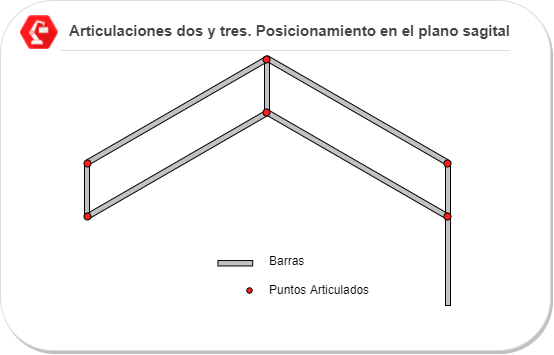
\includegraphics[width=0.75\textwidth]{figuras/mecanismos_4_barras.png}   
    \caption{Esquema de la cadena cinemática correspondiente a los \completarCon{Glosario a GDL} dos y tres}
    \label{fig:Mecanica:4_bar_mecanism}
    \end{figure}

\section{Posicionamiento de sensores y actuadores} \label{sec:Mecanica:sensores_actuadore}

\section{Estudio de la cadena cinemática completa} \label{sec:Mecanica:cadena_cinematica}